% !TEX root = ./main.tex
% !TEX encoding = UTF-8 Unicode
% !TEX program = pdflatex
% !TeX spellcheck = it_IT

\chapter{Analisi dei risultati}
In questo capitolo saranno mostrati i risultati ottenuti per ogni combinazione
lineare utilizzata nel caso delle due differenti soglie di diffusione.

\section{Scelta dei parametri di Scoring}
Per il tuning dei parametri di scoring si è eseguito l'intero processo più volte,
mirando ad ottenere la combinazione che presentasse la copertura maggiore del grafo.\\
In \figurename~\ref{ris_table_mediana} è riportata la tabella contenente i test effettuati
nel caso A.

\begin{figure}[!htbp]
  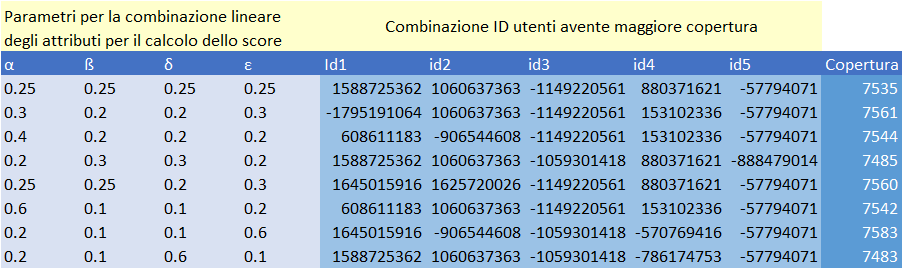
\includegraphics[width=1\linewidth,keepaspectratio]{ris_table_mediana}
  \caption{Tabella Risultati }
  \label{ris_table_mediana}
\end{figure}
\clearpage
In \figurename~\ref{ris_table_media} è riportata la tabella contenente i test effettuati
nel caso B.

\begin{figure}[!htbp]
  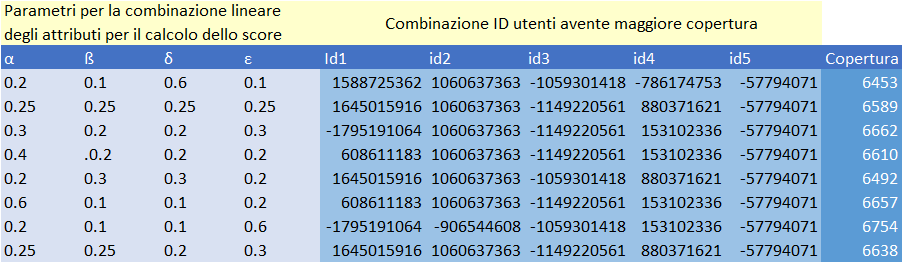
\includegraphics[width=1\linewidth,keepaspectratio]{ris_table_media}
  \caption{Tabella Risultati }
  \label{ris_table_media}
\end{figure}

\section{Risultati}
\subsection{Caso A}

\begin{figure}[!htbp]
  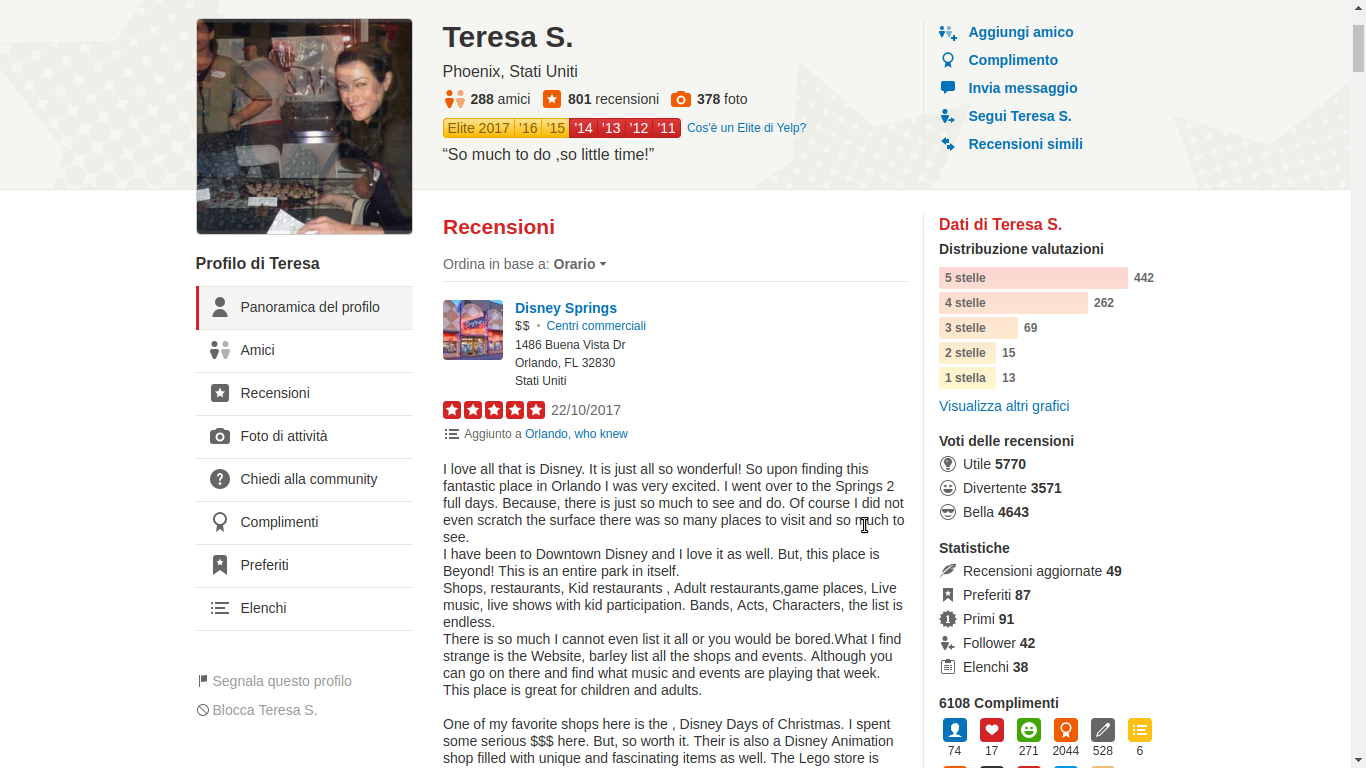
\includegraphics[width=1\linewidth,keepaspectratio]{id1_mediana}
  \label{id1_mediana}
\end{figure}


\begin{figure}[!htbp]
  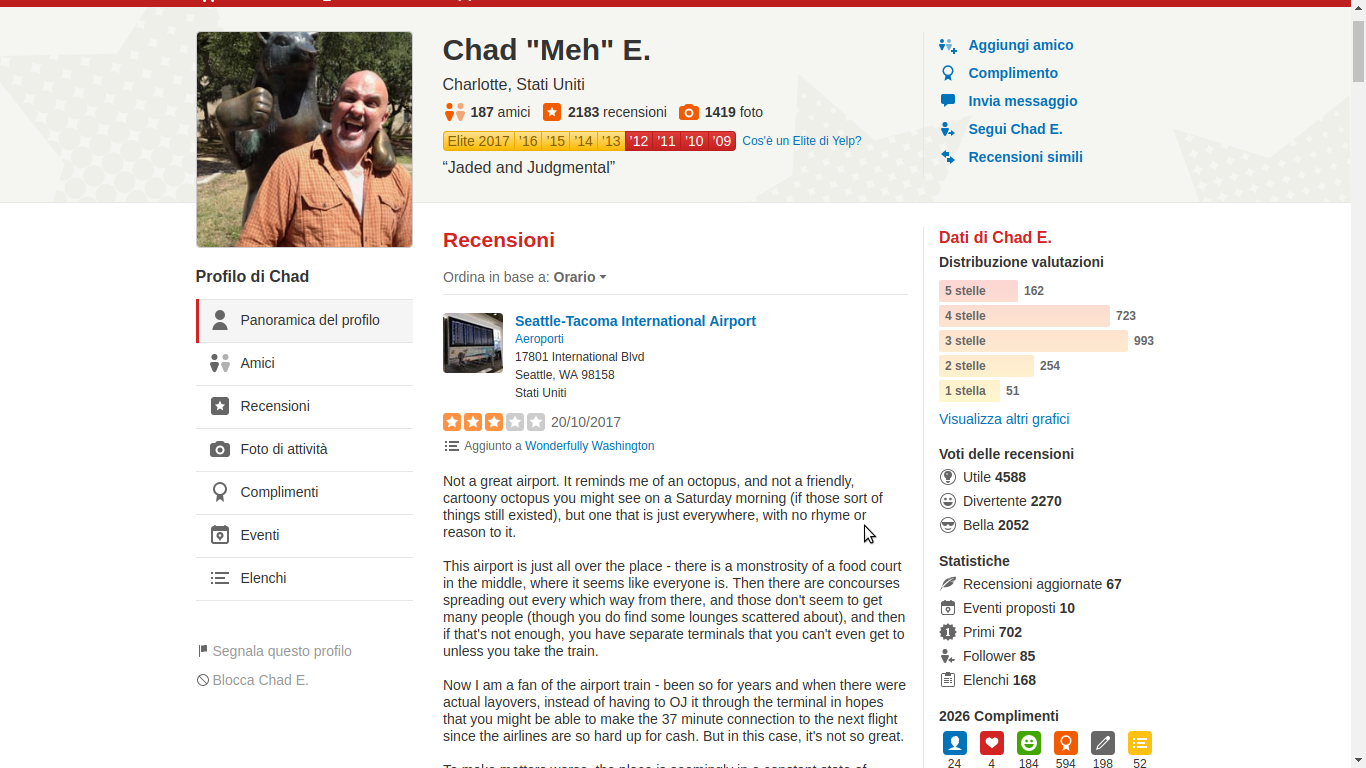
\includegraphics[width=1\linewidth,keepaspectratio]{id2_mediana}
  \label{id2_mediana}
\end{figure}


\begin{figure}[!htbp]
  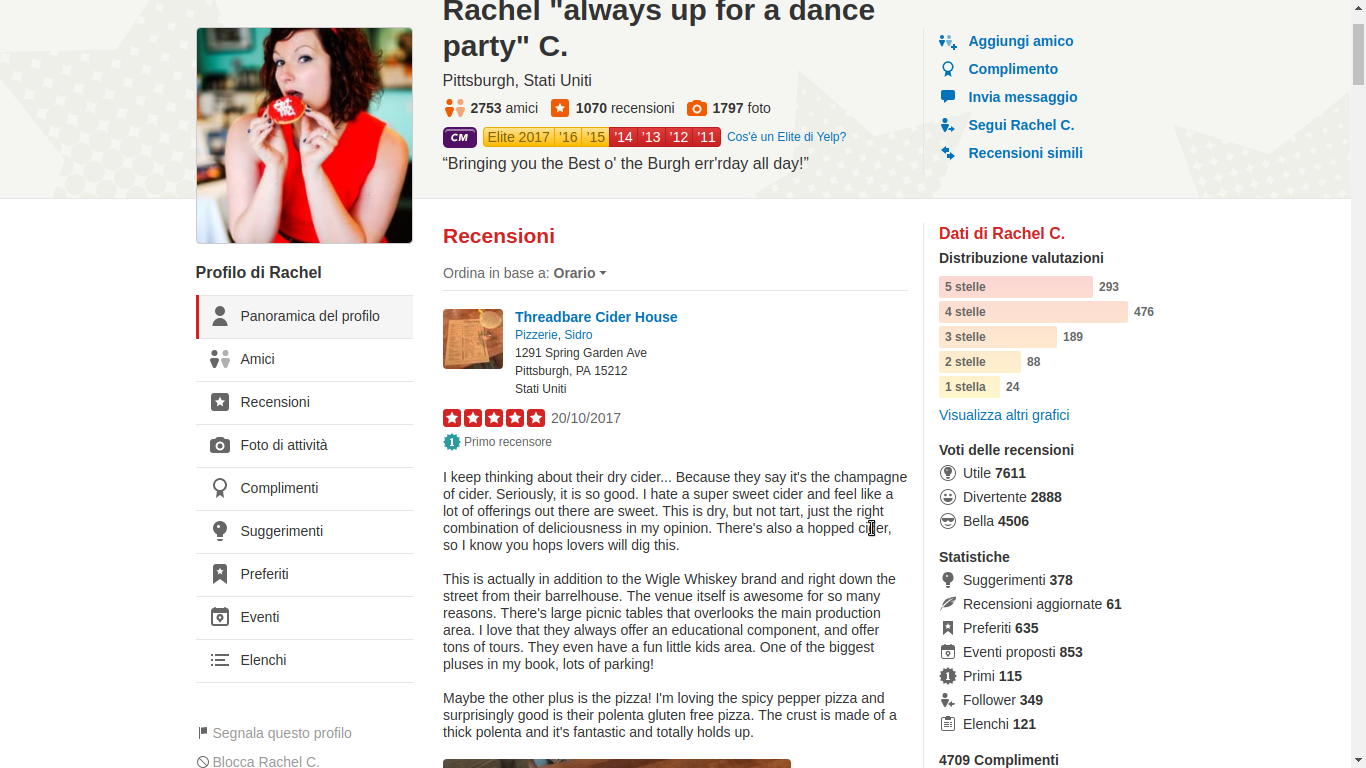
\includegraphics[width=1\linewidth,keepaspectratio]{id3_mediana}
  \label{id3_mediana}
\end{figure}

\begin{figure}[!htbp]
  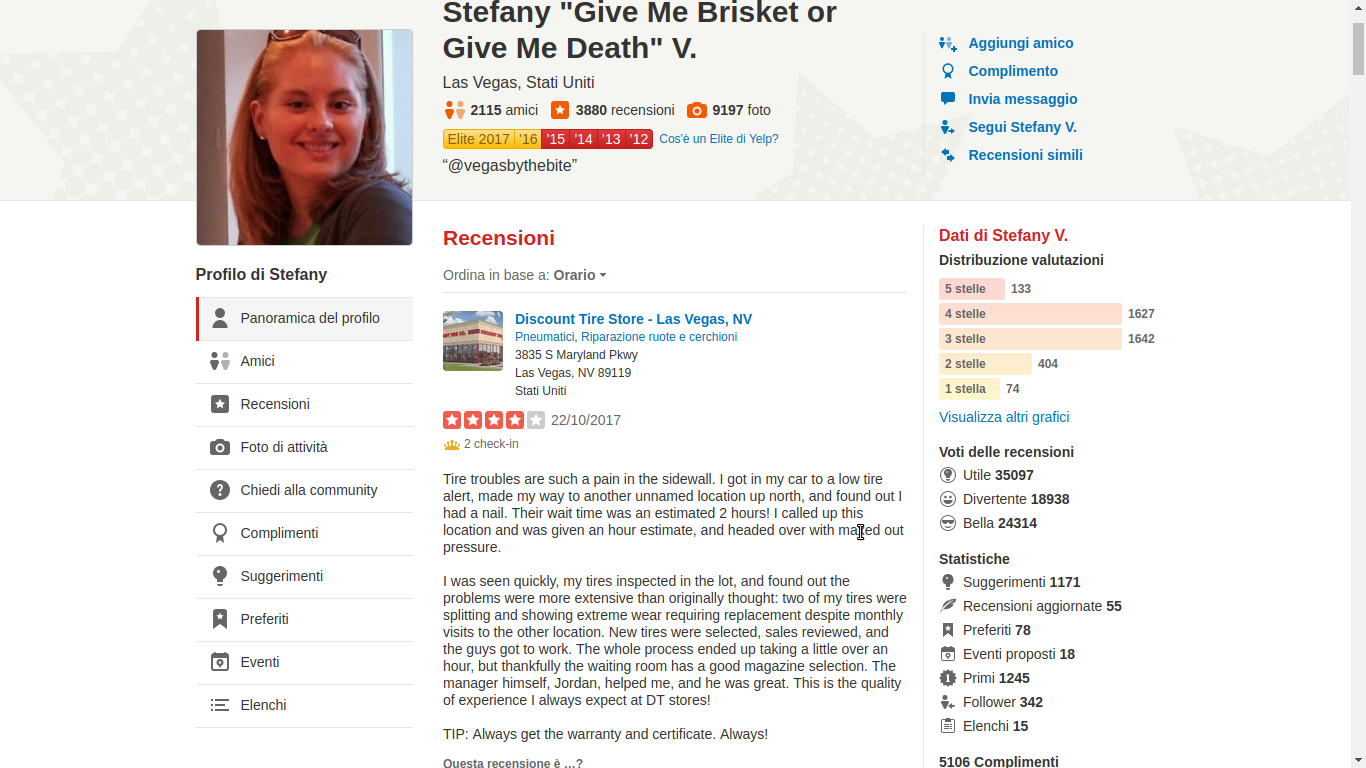
\includegraphics[width=1\linewidth,keepaspectratio]{id4_mediana}
  \label{id4_mediana}
\end{figure}

\begin{figure}[!htbp]
  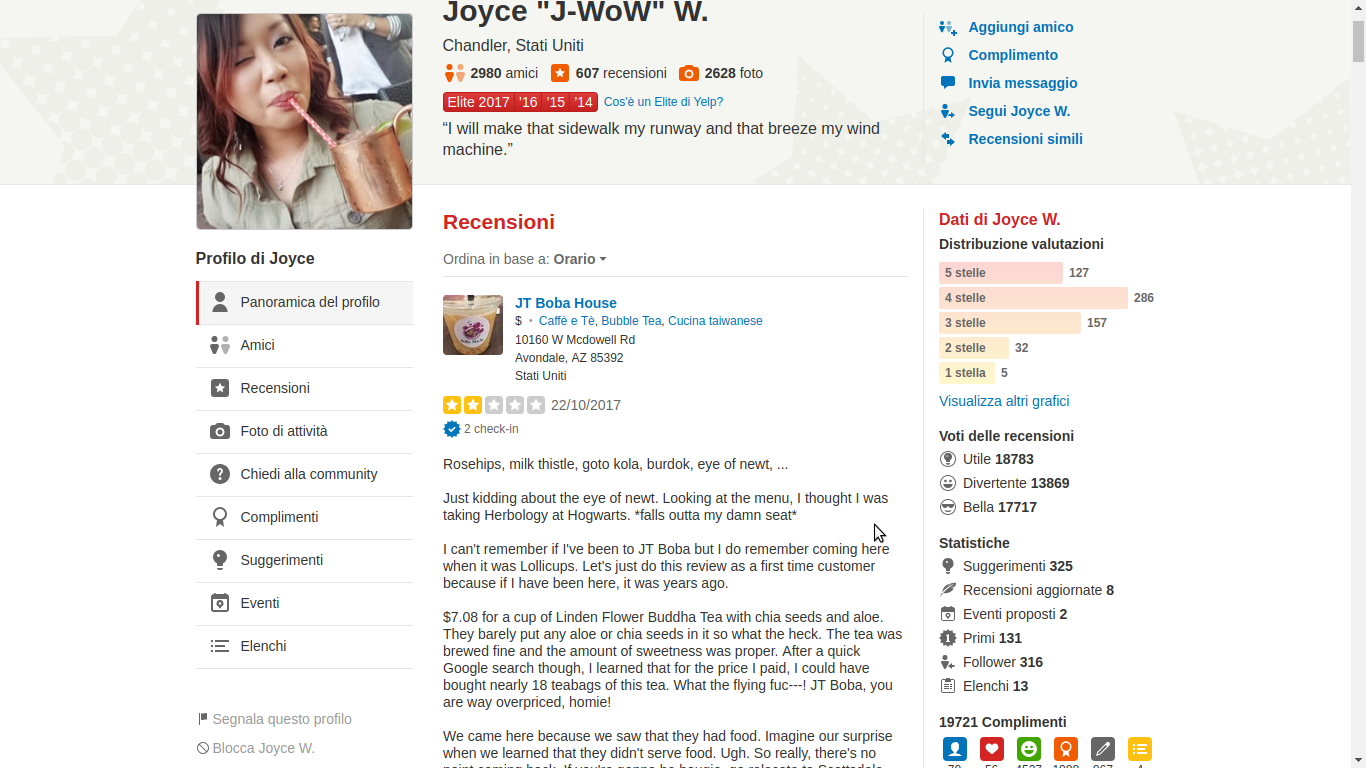
\includegraphics[width=1\linewidth,keepaspectratio]{id5_mediana}
  \label{id5_mediana}
\end{figure}

\clearpage

\subsection{Caso B}

\begin{figure}[!htbp]
  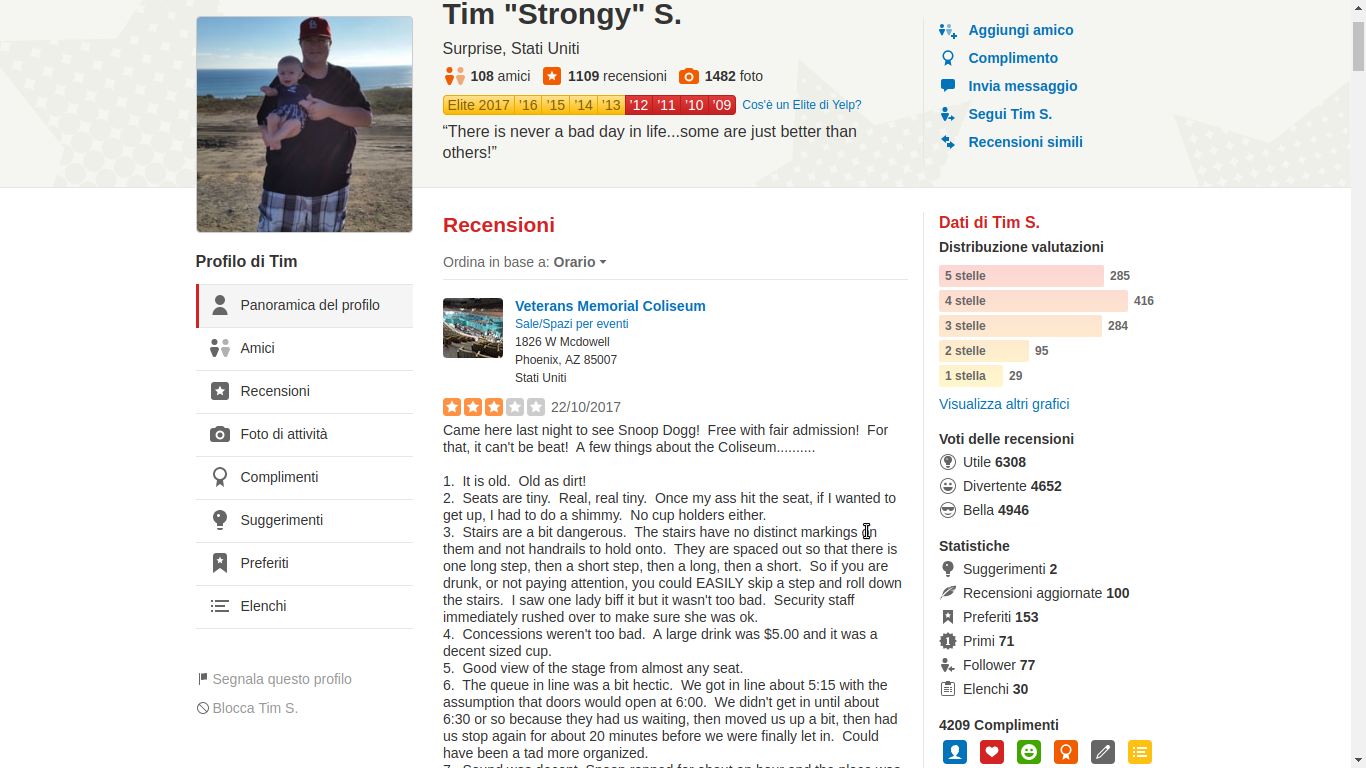
\includegraphics[width=1\linewidth,keepaspectratio]{id1_media}
  \label{id1_media}
\end{figure}


\begin{figure}[!htbp]
  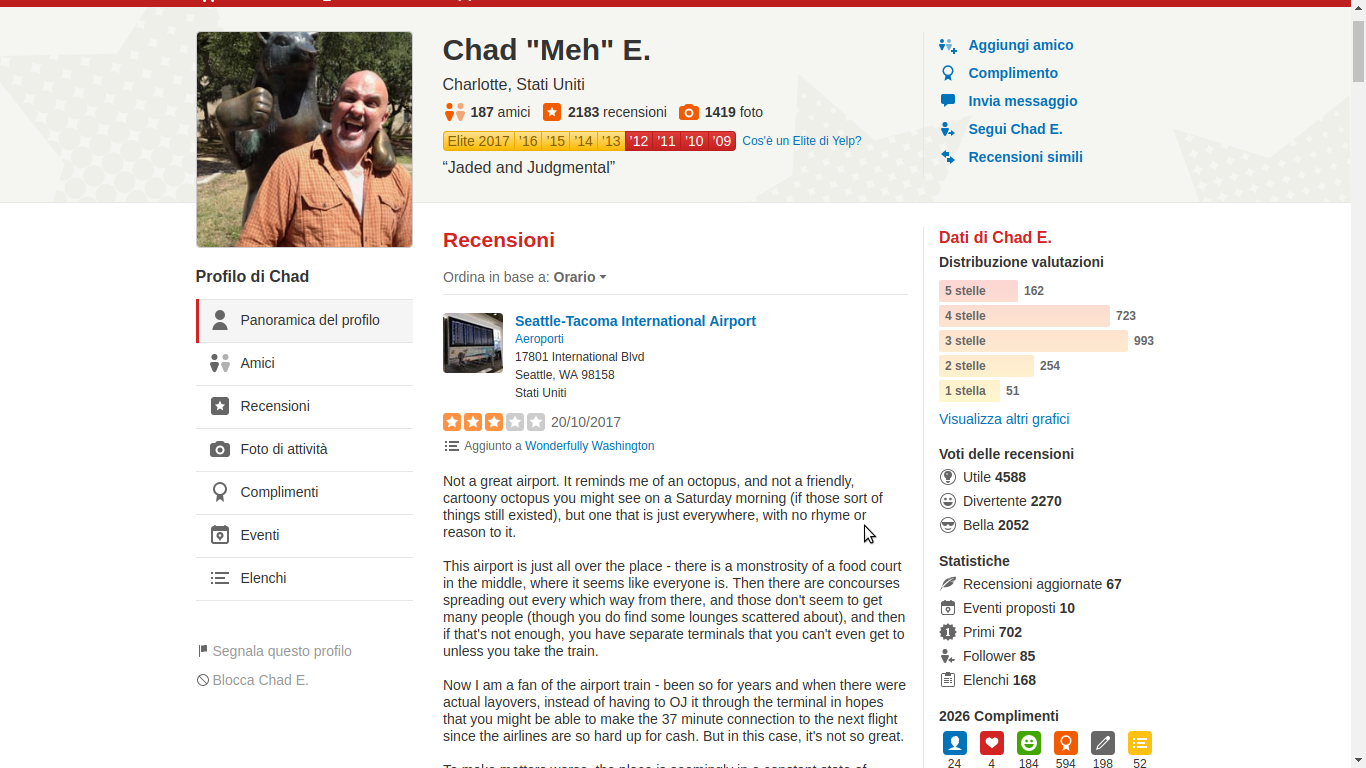
\includegraphics[width=1\linewidth,keepaspectratio]{id2_mediana}
  \label{id2_mediana}
\end{figure}


\begin{figure}[!htbp]
  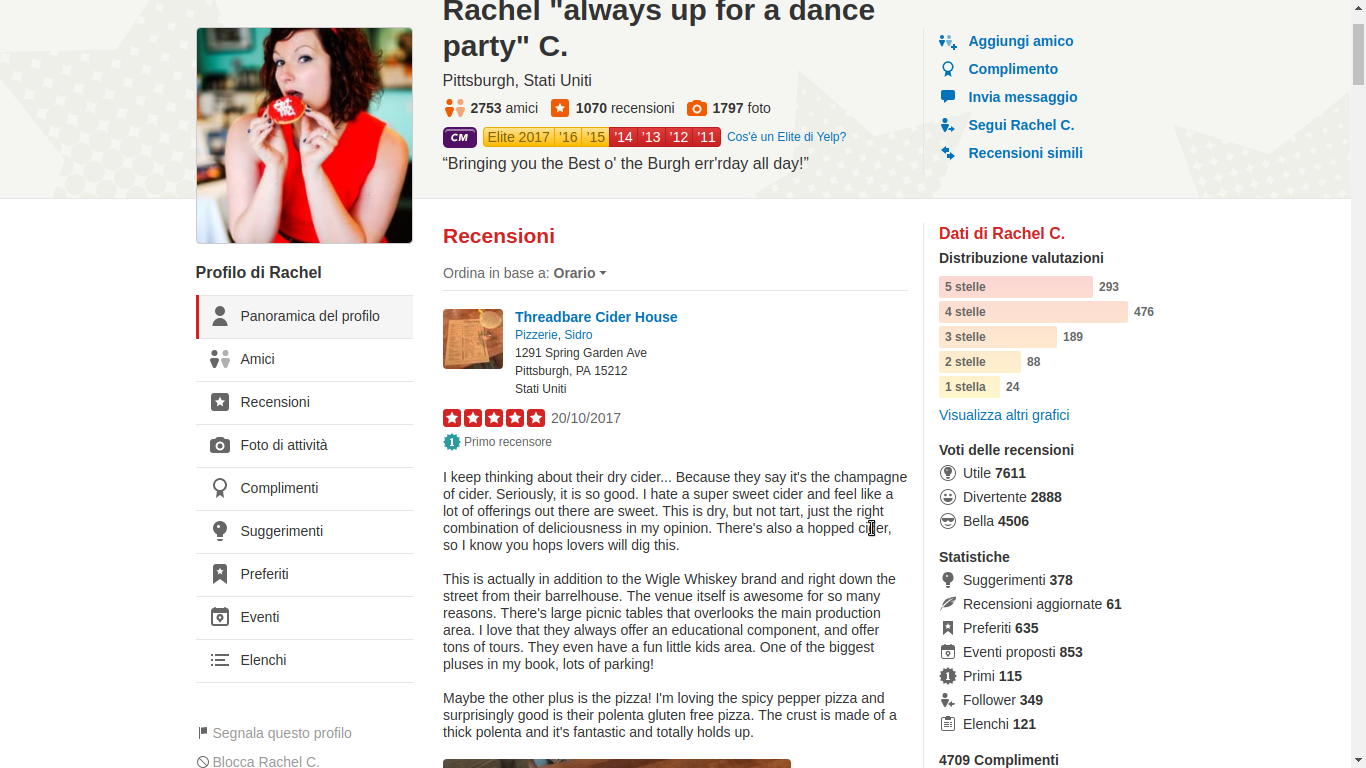
\includegraphics[width=1\linewidth,keepaspectratio]{id3_mediana}
  \label{id3_mediana}
\end{figure}

\begin{figure}[!htbp]
  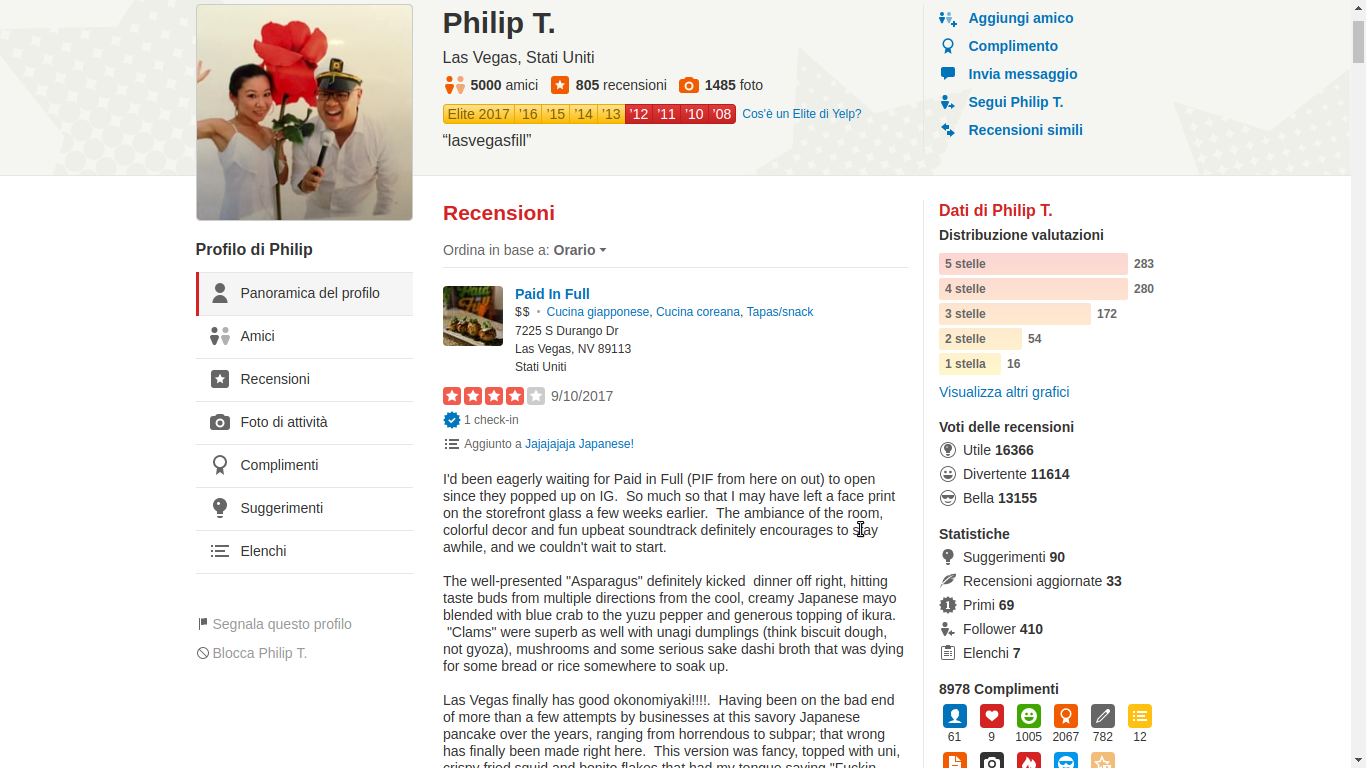
\includegraphics[width=1\linewidth,keepaspectratio]{id4_media}
  \label{id4_media}
\end{figure}

\begin{figure}[!htbp]
  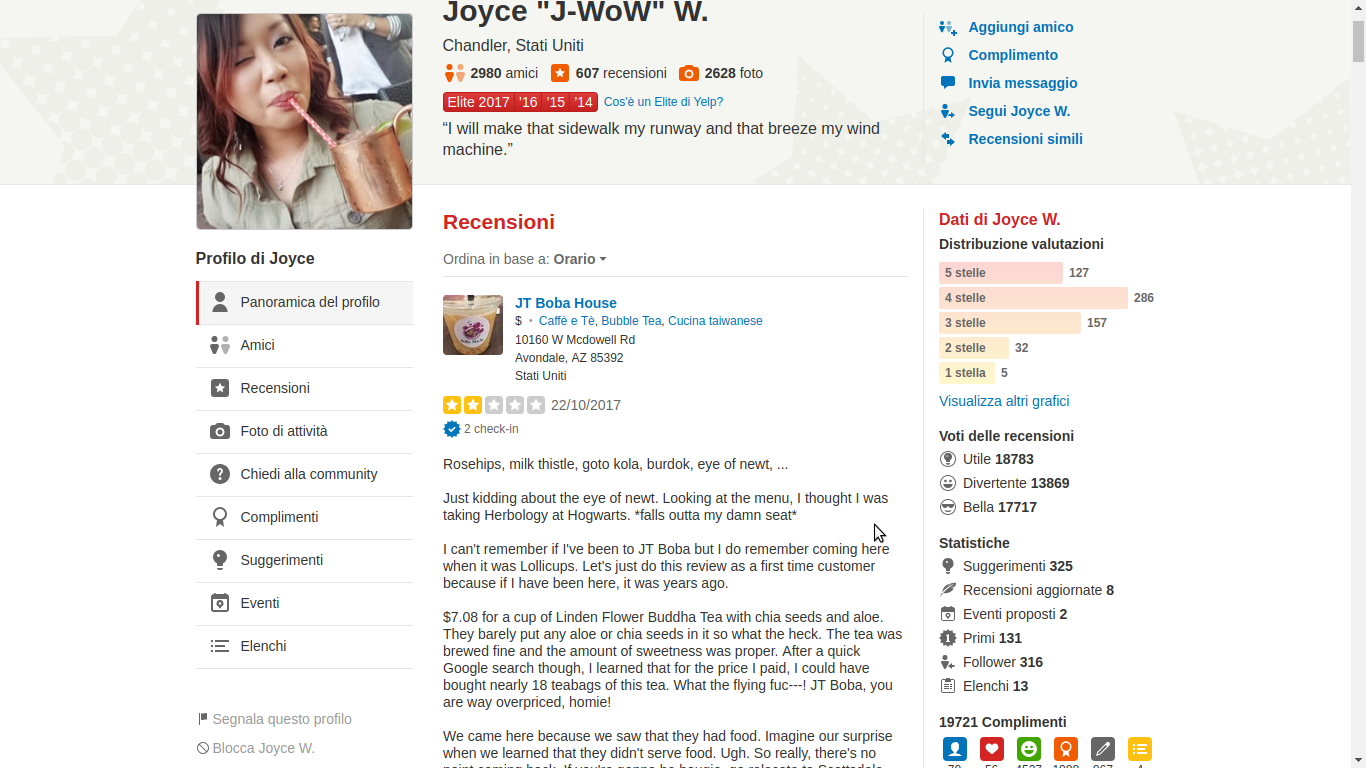
\includegraphics[width=1\linewidth,keepaspectratio]{id5_mediana}
  \label{id5_mediana}
\end{figure}
